The preceding behavioural experiments leave open whether acquired responses remain useful as the material that carries them is produced and lost. We now examine complementary physical evidence and a distinct density-regulated host in which acquisition is tested during actual tissue production. These experiments use distinct inherited rules, acquired bodies and generative implementations; they are not later phases of the cue-learning lives in Figs.~\ref{fig:lifetime-learning} and \ref{fig:temporal-credit}. Their scientific role is to identify actual substrates, costs and constraints for joining learning to renewal. Fixed-physiology results retain their original interpretation; the new host's acquisition is assessed against an explicit non-writing behavioural control.

\subsection*{Inherited tolerance does not identify a benefit from individual experience}

The regenerative experiments ask what kind of body could support continuing adaptation while producing and losing tissue. An inherited rule can change this capacity before any individual learns. We therefore separate the rule package, the initialized body and the consequences of experience. These are distinct sources of a favourable future, even when all are expressed as greater persistence after a challenge.

In a compact lineage, the parent becomes extinct at steps 178, 183 and 177 under the three registered exposure conditions, whereas its offspring remains nonzero through step 224 in all three. Each offspring continuation nevertheless loses mass in its last 32 steps. A rule--initial-state cross places the parental and offspring rules into both initial packages. Finite survival follows the offspring rule in this comparison, including when it is applied to the parental initial package (Supplementary Fig.~\ref{fig:inheritance-recovery}). This supports an inherited change in tolerance over the observed interval. It is not evidence that exposure taught the offspring a more effective response.

The distinction is visible in the experienced-minus-naive returns. For the offspring rule with parental initialization, experience increases final mass by $0.687$ in the specified comparison while lowering final energy by $6.279$ and complete 0--224 body-time by $40.633$. The latter includes acquisition rather than only the final challenge. The rule package contains both interaction kernels and full response parameters; the initial package contains density, intracellular energy, founder labels and polarity. Neither factor can be renamed a pure geometry manipulation. The observed survival effect is therefore a property of a complete inherited physiology in its tested context.

The same direction does not generalize to a multiring lineage. Its offspring performs worse than its parent in all six matched continuations, and replacing the parental rule by the offspring rule is adverse under both initial packages. Complete experienced-minus-naive body-time is negative in both offspring lineages. These results retain the compact lineage's conditional positive tolerance without converting it into a general rule-improvement or experience-adaptation claim. They also illustrate why selection history matters: a later complete ranking of offspring cannot turn an earlier continuation of a partially selected candidate into a prospective test of that full ranking.


Recovery after a physical cut provides another distinction. An independent receiver branched at step 256 regains total mass while the original cut region remains depleted and later shrinks. The spatial reference is the same original-coordinate region, not a region recentered on the surviving body. Total production elsewhere is thus insufficient evidence of local restoration. A compact receiver in the corresponding set becomes extinct at step 273. These comparisons motivate separating maintenance, repair, learned avoidance and inherited tolerance rather than combining them into a single recovery score. Evolution and development can supply useful embodied capabilities\cite{gupta2021,kriegman,duran,colizzi}; demonstrating how an individual changes its behaviour requires the within-body controls used above.

\subsection*{Fixed physiology can support genuine finite tissue replacement}

A finite positive replacement result is available without learning or a new deletion policy. We initialize compact, ring, double-lobed and separated bodies under the same selected generative rule, with two new fixed input tapes. For each seed--shape parent, the original greedy response policy is compared with a uniform one-hop redistribution of the rule's deletion requests. Initial density and intracellular energy are supplied at life zero; the ring is prescribed as a ring. It is not a ring learned or generated from a compact founder during the experiment.

Both ring seeds satisfy the registered maintenance criterion in every one of four consecutive 64-step windows under both policies (Supplementary Fig.~\ref{fig:finite-replacement}). The result is unchanged when numerical tolerance is reduced from $10^{-8}$ to zero. The original greedy rule already possesses this finite capability, so the deletion-layout modification is not a necessary explanation. All other twelve trajectories fail the final two-window criterion. The positive finding is therefore specific to the ring initializations and the tested finite protocol, not an average across successful and unsuccessful shapes.

Material labels show that the ring result is more than keeping the initial body intact. Initial founder mass is 64; by step 256 its surviving contribution is approximately 35.98--36.87. Tissue born after life zero contributes 35.307--35.690 at the endpoint, including approximately 21.949--22.068 born after step 128. Replacement is physically realized while a substantial fraction of founders disappears. This is a stronger observation than a nonzero final body or cumulative positive birth, but it remains limited to 256 steps. Four successful finite windows do not establish an indefinitely maintained steady state.


Deletion layout also produces conditional improvements that should not be overstated. In the life-zero comparison, uniform redistribution improves the jointly screened mass, energy, body-time and post-128 tissue outcomes only for the compact and double-lobed pairs. Ring and separated bodies lose mass and body-time relative to the original policy. Across all eight paired conditions, post-128 retention is positive in six and negative in two. A positive average would obscure those failures and would not justify incorporating uniform redistribution as the default generative rule.

In a separate intervention on already acquired states, both mass-weighted and uniform one-hop deletion layouts increase final mass, energy, body-time and true post-256 tissue in all four related contexts. Uniform redistribution gives mean differences of $0.286$, $0.721$, $1.256$ and $0.227$, respectively. Yet all twelve trajectories in that experiment fail the two-window maintenance screen and have negative birth-minus-death in the last 64 steps. The actual total deletion requested by the original rule is preserved at each intervention state; subsequent cumulative deaths may differ because the future bodies diverge. Additional coordination is externally supplied and not physically priced. These observations identify an effect of deletion location within a given physiology, without identifying a learning process or a general maintenance solution.

The juxtaposition matters for the main question. Some fixed bodies already replace tissue over the available window, whereas some interventions improve several totals without achieving even that limited maintenance result. The desired learning body need not surpass its control on every physical variable, but it must have a viable material substrate on the timescale over which its acquired behaviour is evaluated. The ring positive provides one such finite substrate. It is not yet the conservative cue-learning body, and no result here shows acquired cue values surviving the ring's replacement process.


\subsection*{Conditional acquisition can coexist with real tissue production in a different host}

The finite ring result does not itself join behaviour to renewal. We therefore distinguish a further, explicitly different material CA in which local density regulates birth and death while an installed central controller reads acquired cue values. This model preserves paid material transport and local birth admission, but its generation rule is not the original Lenia kernel response. Extracellular stocks receive measured external supply. It is a reusable experimental host for behavioural questions about real tissue production and loss, rather than evidence that the earlier Lenia rule or the local non-renewing motor body has acquired these capabilities (Fig.~\ref{fig:young-turnover}).

The behavioural question also requires separating experienced consequences from direct tissue selection. In preceding injury-based tests, continuing value updates improves safe contact relative to retaining stale values, but resetting those values without further writing reproduces much of the improvement. A fixed prior can pass acquisition. These controls prevent attributing the entire difference to a newly learned useful response. The subsequent energetic task changes the local consequence: actual uptake is followed by an energy tax that enters heat rather than directly deleting tissue according to cue identity. Feedback uses completed uptake minus the amount of tax actually paid. Real physiological death, starvation, birth and transport remain possible; the condition is not a physically lossless learning model.

Two opposite meanings are applied to each of two supplied initial geometries. In the compact geometry, a standard current-feedback update acquires the favourable response in both conditions, while the matched fixed prior does not. Final-64 safe-contact fractions are $0.81632$ and $0.76208$, versus $0.58561$ and $0.60644$ with the fixed prior; absolute safe-contact masses are $75.136$ and $68.963$. At the acquired step-256 checkpoints, $83.225\%$ and $83.700\%$ of the actual body is material born after life zero. This establishes conditional acquisition alongside substantial real tissue production in that same implementation. It does not establish that copying the acquired content into new material explains the behaviour. Net growth accompanies birth and loss, so the newborn fraction is not a one-to-one fraction of founding tissue replaced.

The alternative elongated geometry provides two acquisition counterexamples. Neither compact condition passes the registered final reversal window after the outcome meaning changes, and the elongated conditions fail that reversal criterion as well. Among the later compact stop-writing endpoints, only one fast condition passes. Four elongated main paths lack their planned 128-step terminal segments after a storage stop; these missing windows remain unavailable, not zero-valued failures or successful continuations. The original same-parent future-writing controls and all fixed-prior results remain in Supplementary Table~\ref{tab:young-phases}. Neither opposite meanings nor initial geometries are treated as independent random replications, and the conditional acquisition is not a new-method advantage.

To test newborn content more directly, each of the two qualifying complete step-256 compact parents branches for 128 updates with new writing disabled and the acquired meaning unchanged. Actual newborn tissue receives the local pre-write copy, a zero payload under the same tariff, or a norm-preserving swap of cue contents. Surviving old content is untouched and all initial physical states and histories match. Physical uptake and energetic feedback continue: this is stop-writing expression, not no-feedback retention. Tissue born during the probe comprises $58.798\%$--$60.466\%$ of its final body. All six branches retain the registered safe-contact behaviour. In the first parent, all three physical and action histories are exactly equal despite nonzero content differences. In the second, safe fractions are $0.83241$, $0.83326$ and $0.82582$ for copy, zero and swap; action differences occur without changing the passing outcome. Thus correct newborn copying is not necessary in this tested window. It does not follow that all inherited content is irrelevant: old tissue remains and its contents are not erased.

The joint interpretation is deliberately architectural. Original Lenia generation, conservative local motor learning and this externally supplied density-regulated birth/death model answer different questions. The last now demonstrates standard conditional acquisition during tissue production, whereas the local-motor experiment demonstrates content-dependent action without birth. Neither yields the full repeated revision and maintenance of useful experience through turnover. Their costs and negative controls specify what an integrated explanation must account for, without combining separate hosts into one continuous adaptive life.

\begin{figure}[p]
\centering
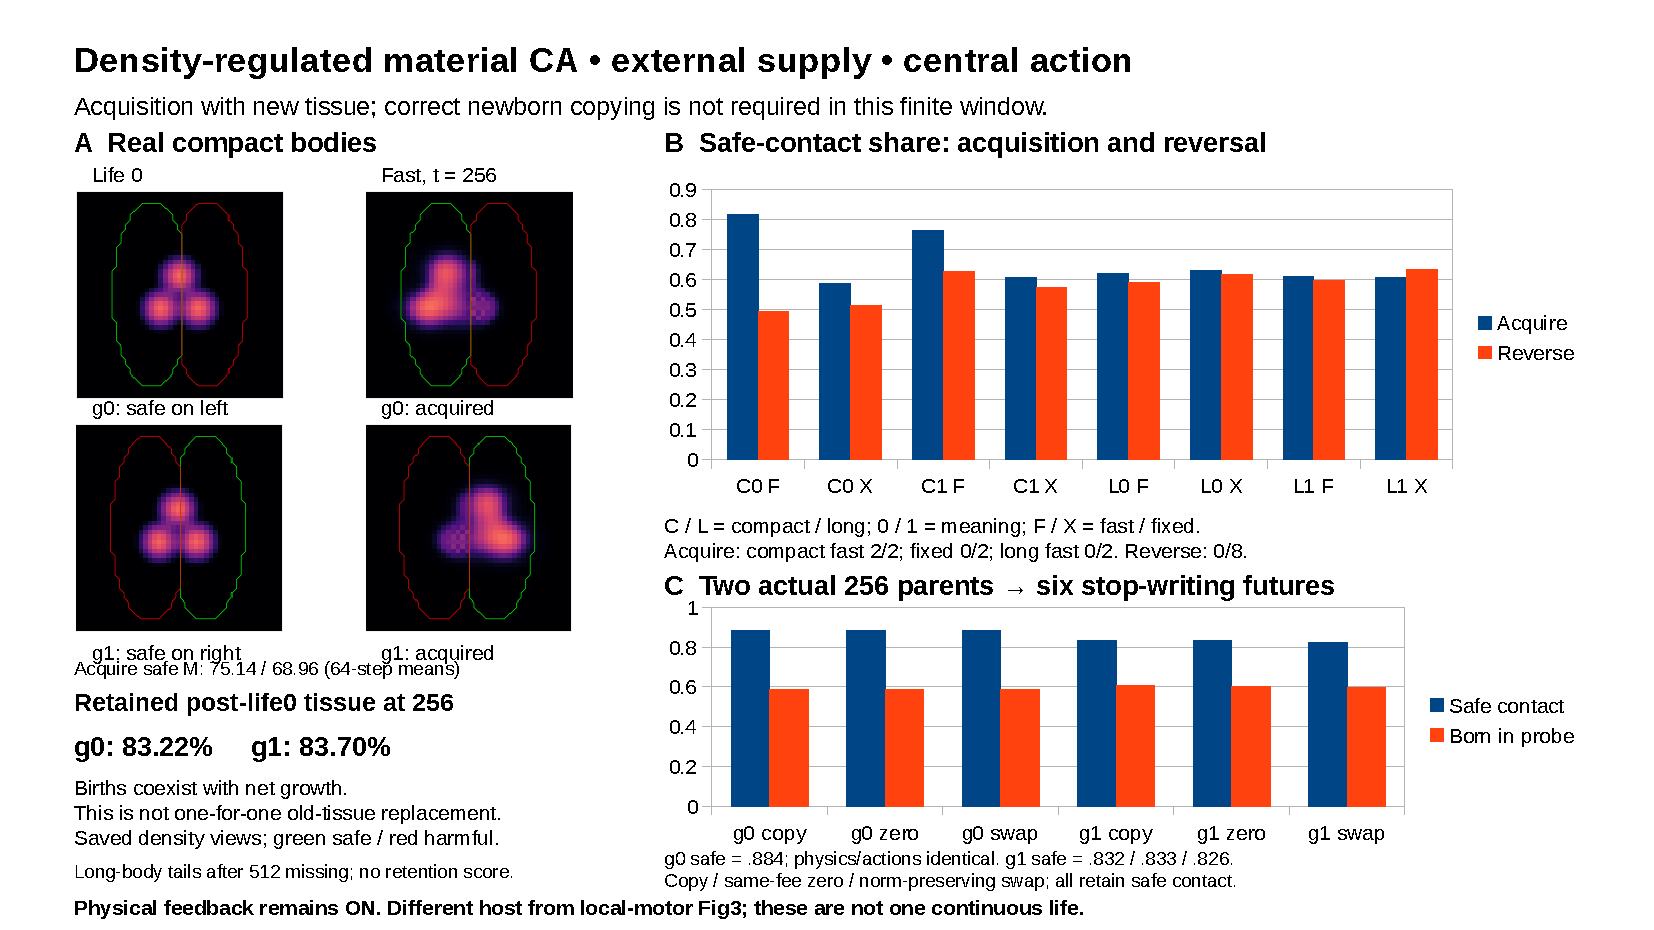
\includegraphics[width=\linewidth,height=0.72\textheight,keepaspectratio]{work/longform_v047/figures/young_turnover_v0475/young_turnover.pdf}
\captionsetup{font=footnotesize}
\caption{\textbf{Conditional acquisition during real tissue production in a distinct host.}
\textbf{a}, Actual compact density fields at life zero and acquired step 256. Green/red contours mark safe/harmful regions; these are density views, not spatial birth-cohort maps. Post-life-zero tissue constitutes $83.22\%$ and $83.70\%$ of the two acquired bodies. Births accompany net growth, so these shares do not measure one-for-one founder replacement.
\textbf{b}, Final-64 safe-contact fractions for all eight geometry--meaning--controller conditions. Compact fast acquisition passes $2/2$, compact fixed prior $0/2$, elongated fast $0/2$; all eight fail complete reversal. Success also requires absolute contact, viability and tissue criteria. The elongated expression tails after 512 are missing.
\textbf{c}, Two actual acquired parents each provide copy, same-tariff zero and norm-preserving swap futures. Writing stops for 128 steps, while physical energetic feedback continues. Safe contact is a final-64 mean; born-in-probe bars are endpoint retained fractions. All six related futures pass; the first parent's physical/action histories coincide. Correct newborn copying is therefore unnecessary in this tested window, with surviving old contents intact. This externally supplied density-regulated material CA has central action and differs from both original Lenia generation and the no-birth scalar-action host in Fig.~\ref{fig:scalar-action}.}
\label{fig:young-turnover}
\end{figure}




\subsection*{Sequential resource admission produces distinct mass and energy effects}

Regeneration depends on what a body can actually admit, not merely what its response function requests. In the resource experiments, a positive generative request passes through capacity and template constraints and then through precursor P and fuel F availability. We independently enable the registered transport capabilities in two acquired bodies, a porous form and a four-lobed form. Their first post-branch action is especially informative because the body, actual transport, licensed request and template support are still matched before the resource-admission paths separate.

At action 129, enabling P transport increases the requested mass subsequently rejected by F from $0.0786$ to $0.2863$ mass units in the porous body and from $0.1219$ to $0.2434$ mass units in the four-lobed body. The available F field is identical pointwise, and the independently evaluated F deficit remains unchanged, at $11.4326$ and $2.1079$, respectively. More requests reach the F constraint because the preceding P constraint has admitted more of them (Fig.~\ref{fig:allocation-feedback}). Increased downstream rejection therefore does not imply that the fuel supply itself became worse.

This is a general interpretive issue in a sequentially constrained system. A change in the mass rejected at one constraint can reflect the requests admitted by upstream constraints. The P and F deficits overlap and cannot be summed as independent lost masses. A scalar rejection amount would consequently be an ambiguous objective for an adaptive controller. The appropriate measurements include the admitted material, energy expenditure and the state on which each constraint acted, not just the rejected amount.

\begin{figure}[p]\centering
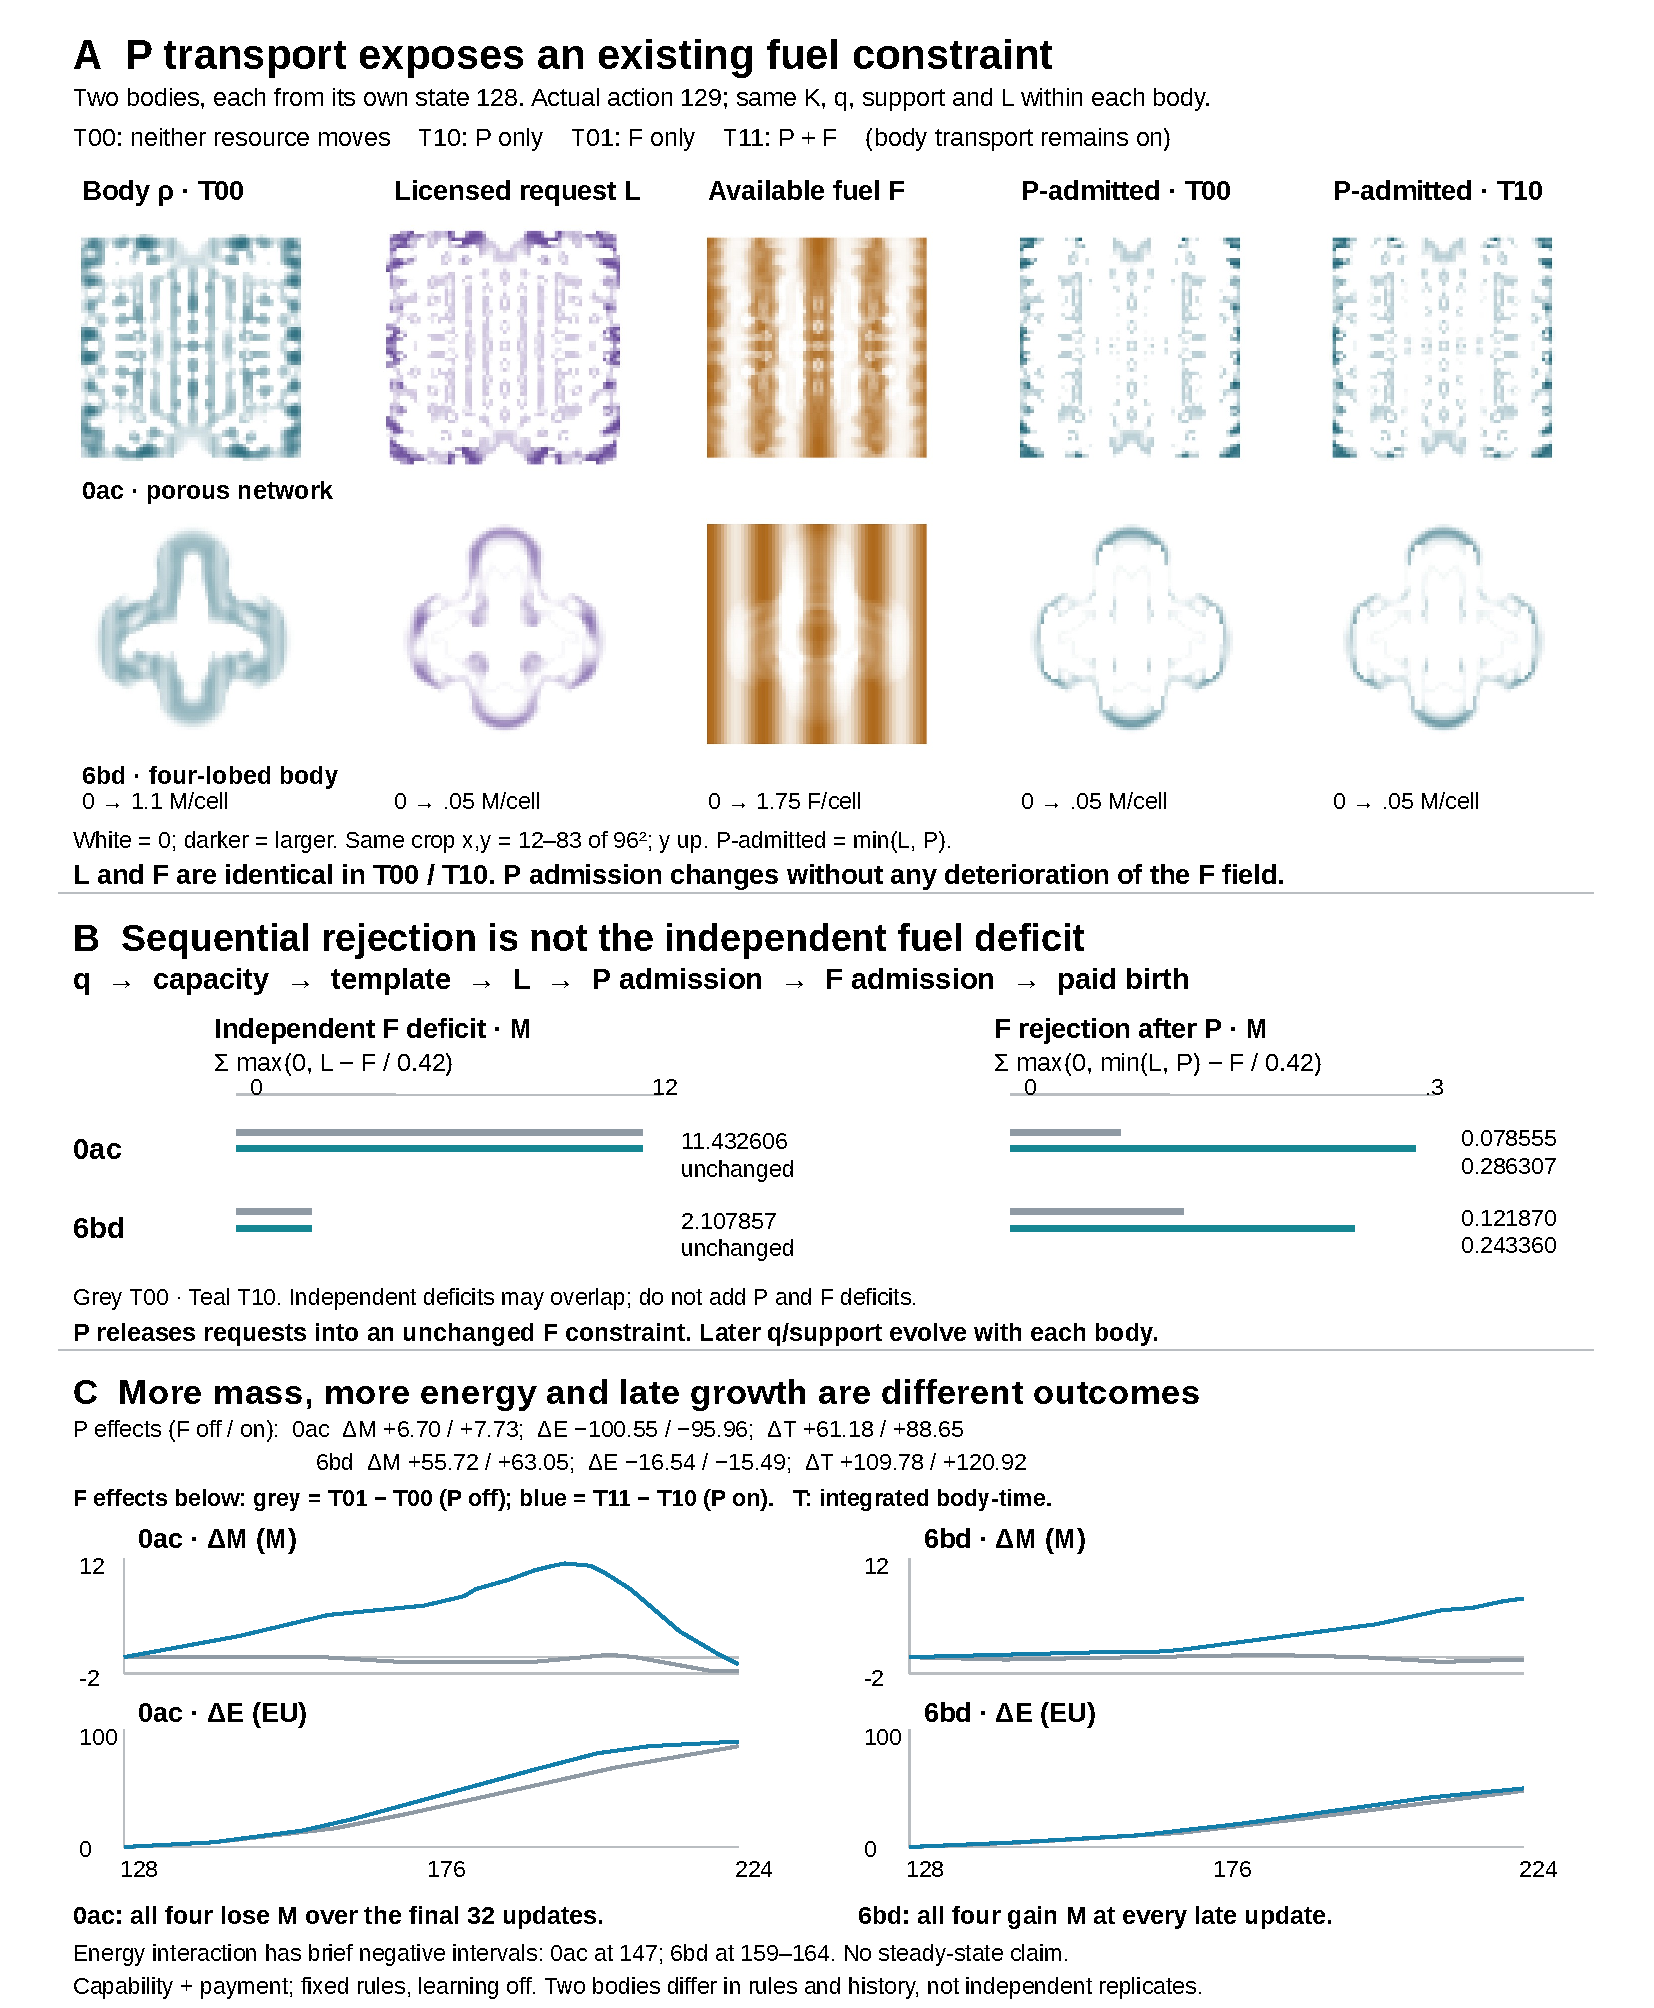
\includegraphics[width=\linewidth,height=.75\textheight,keepaspectratio]{figures/main/resource_constraints/resource_constraint_unmasking.pdf}
\caption{\textbf{P transport exposes fuel constraints without worsening fuel supply.}
\textbf{A,} Actual action 129 fields in two bodies continued from their own state 128. Fixed original-coordinate windows show T00 reference density, common licensed request $L$, common available fuel, and P-admitted requests with P transport off/on (T00/T10). Within each body, $K$, $q$, template support and $L$ match; F is identical pointwise.
\textbf{B,} The sequential capacity--template--P--F rule exposes more F rejection when P admits more requests, although the independent F deficit is unchanged. The quantities use separate scales; overlapping P/F deficits must not be added.
\textbf{C,} P increases final mass and body-time while reducing energy. Full-window F effects increase energy but change mass differently across bodies and time. All four 0ac branches lose mass over their final 32 updates; all four 6bd branches grow at every late update. Energy interaction is briefly negative despite positive endpoints. Capabilities and their actual payment change together; rules are fixed and learning is off. This is a conditional resource comparison, not an experience-adaptation test.}
\label{fig:allocation-feedback}\end{figure}


Over the subsequent window, P transport increases final mass and integrated body-time but lowers final energy. F transport raises energy throughout the tested interval, whereas its effect on mass depends on body and time. All four porous branches lose mass over their last 32 updates; all four four-lobed branches grow at each of those late updates. Even when endpoint interactions are positive, some energy interactions are briefly negative. Actual small starvation losses and the transport payments are retained in these accounts. No steady-state claim follows from the four-lobed late growth.

The matched first action permits a narrow mechanism statement about exposed constraints. It does not fix the organism over the entire future. Later density, templates, resource fields and transport masks differ, so a long-horizon effect cannot be interpreted as a single resource mediator acting in otherwise identical tissue. Capabilities and their actual costs change together. The experiment uses fixed rules with learning disabled; its role is to explain the physical opportunities and trade-offs that a future learner must control.

This distinction complements work on adaptive transport and collective resource organization\cite{tero,teronetwork,liu,prindle}. Such systems can show useful distributed organization without an explicit trial-based learning rule. Here, the accounting makes clear which resource constraint has changed and which consequences arise only after the body develops differently. It also supplies a reason to keep behaviour and viability separate: more tissue can be purchased with less residual energy, and less immediate growth can preserve fuel for a later useful action.

\subsection*{The value of physical effort depends on the body and the time window}

A complementary intervention tests an action cost directly, without changing a learning rule. Four actual acquired parents, two compact and two softer bodies with different prior directional conditions, are continued from clock 1984. Each receives a resource field of width 1.6 or 4 and either the original propulsion amplitude or half that amplitude, giving sixteen 128-update futures. The amplitude change is applied before the controller's inverse mapping; checks of the actual transport and displacement confirm that it changes the physical action rather than being cancelled by normalization. No new acquisition is run and no policy learns which width or effort to select.

Halving effort reduces paid movement expenditure and total uptake in all eight within-parent, within-width comparisons (Supplementary Table~\ref{tab:effort-comparisons}). The energy consequence differs between bodies. Compact-body uptake losses of $0.5633$--$0.9276$ exceed the savings sufficiently to lower final energy by $0.1669$--$0.5295$. Softer-body uptake losses are smaller, $0.0368$--$0.1133$, and final energy instead rises by $0.1110$--$0.1972$. Final mass and integrated body-time nevertheless decline in all eight comparisons. All sixteen futures remain viable under the registered minimum-mass criterion; these measured trade-offs are neither uniform improvement nor a failure merely because one physical quantity falls. The two resource widths do not reverse the energy ranking. This comparison therefore supplies no evidence that different width histories have been learned or that historical information is required to choose between the tested efforts.

Time and spatial resolution change the interpretation of the totals. In the softer bodies, half effort raises uptake during the final 64 updates by $0.0153$--$0.0436$ across the four comparisons, but total uptake over all 128 updates remains lower. The late benefit does not recover the earlier loss, and nested windows are not new independent trials. Moreover, greater total energy need not protect every part of a body. Under the wider resource field, the softer half-effort bodies contain $0.0727$ and $0.0692$ mass units below the registered local energy-per-mass threshold of $0.08$, compared with $0.0093$ and $0.0252$ under full effort, despite higher mean energy per mass. This coexistence identifies a spatial limitation of the global reserve measure; it does not isolate local energy deficiency as the cause of tissue loss.

The physical comparison thus asks what an eventual learner would have to value, not whether an adaptive controller has already learned that valuation. Even with all movement charges paid, lower effort trades access to supply against expenditure and local distribution. An analytical bound obtained by freely relocating extracellular supply is an unattained opportunity under an external intervention, not a realizable control benefit. Full costs, unpaid basal requests, resource stocks and early/late windows remain available alongside the paired outcomes (Supplementary Table~\ref{tab:effort-costs}). Distinguishing an opportunity from an experienced improvement is necessary before history-dependent action can be credited with exploiting it.

\subsection*{Production, retention and the location of material have different consequences}

The same separation is necessary when evaluating attempts to renew tissue. A trained resource-conditioned generative policy initially fails to produce a qualifying nonzero proposal in two rounds of outer search. A strong pre-state greedy policy improves final mass, energy, body-time and actual post-128 tissue relative to the deployed constant response, but most of the gain comes from keeping older material. Its first 64-step window passes the local maintenance screen; its later windows do not. Neither the search procedure nor the short-window improvement establishes lifetime learning or sustained replacement.

A later third-response comparison supplies a finite positive. Conditional use of the additional response enables both tested shapes to pass all four maintenance windows under the selected policy and a fixed midpoint comparator. The outer two-parameter search does not outperform that simple comparator jointly: selected policies retain more post-256 tissue but have lower final mass, energy and late body-time. Constant use of the additional response causes the two validation bodies to become extinct at steps 173 and 145. The useful result concerns conditional response selection within a fixed physiology; it is not evidence that the individual trained itself during deployment, or that cross-entropy search is a new learning algorithm.

Factorial removal of generative and non-increasing response choices clarifies their interaction. Retaining both classes passes the two-window maintenance screen in all four conditions, whereas the generative-only policy passes none. The latter actually produces more tissue in all four but also deletes more new tissue. In separated bodies, preserving the non-increasing choices supports both older material and more genuinely post-256 tissue. In rings, part of the benefit is older-material preservation. Thus non-increasing choices cannot generally be described as obstructing renewal. Conversely, the non-increasing-only policy is not sufficient for replacement in all conditions. The positive interaction is a difference between complete dynamically changing policies, not a mediator fraction or a fixed local action value.

Direct postbirth continuations resolve some of this ambiguity. At step 320, acquired bodies are branched between the both-class and generative-only futures. We label older tissue $O$, tissue born during 257--320 and still alive at 320 as $C$, and actual births during 321--384 as $N$. The denominator for $C$ is fixed at the branch. Adding both-class support after generative-only history improves $C$ survival in all four parents, but passes the original complete useful-renewal screen only in the two separated bodies. The ring futures have slightly less $N$. Removing support after both-class history also reduces $C$, but the benefit to $O$ is larger; this does not establish a general young-tissue-specific effect. The future both-class branches pass the single observed 64-step maintenance window, which must not be substituted for an earlier two-window criterion.

Age-resolved reconstruction changes the interpretation of lower $N$. Comparing retention at fixed ages 1, 4, 8, 16 and 32 on common birth-clock support, the both-class policy has higher aggregate retention in 39 of 40 parent--age summaries under two common weighting schemes. The exception and 293 negative individual contrasts among 2,072 clock--age comparisons remain in the record. An exact symmetric decomposition gives a positive retention term in all eight endpoint comparisons. In six, including all rings, a larger negative birth-amount term leaves less final $N$. Lower new-tissue stock can therefore coexist with mostly improved age-matched retention. This is an accounting identity across different births in diverging bodies, not an intervention on the same newborn material and not a causal mediation analysis.

Spatial-source accounting supplies a further constraint. For both 16- and 64-step horizons, every parent has some starting sources whose material survives better under the generative-only policy, despite greater total $O$ and $C$ retention under the both-class policy. At 64 steps those adverse-source regions contain 21.88--38.04\% of the initial mass. The cohort differences follow their source weights; they do not establish an intrinsic age-selective policy. Nor does a map of which complete policy performs better at each origin justify stitching their actions together cell by cell. The map conditions on each policy's whole coupled future.

These distinctions also explain the negative controls on more elaborate response semantics. Averaging after rather than before the nonlinear response increases final $N$ in all four parents but reduces existing $C$ in all four; the joint useful-renewal screen fails throughout. Transporting a ready-state response choice with actual material also fails that screen in all eight parents, with lower final $C$ in seven and higher $N$ in only three. The channels are regenerated and discarded each step, with no persistent writer. Material association and convex response mixing change together, so their effects cannot be attributed to a reference-frame change alone. Full results, fees and original screen decisions remain in the indexed Supplementary Information. These failures narrow proposed control mechanisms without redefining a general adaptive behaviour as a vector of nondecreasing bodily totals.

\subsection*{A state can cross replacement without remaining necessary for persistence}

In a separate carrier experiment, we ask whether a locally carried protection state can outlast the tissue in which it was initially present. This is a carrier experiment, distinct from acquiring and reversing a cue preference. In an unequal-peaks receiver, further induction is disabled and the protection state is copied through paid generative events. All tissue present at cutoff 128 disappears by step 205, while the tissue-weighted protection load remains nonzero. At step 384 the retained-copy branch has mass $7.3366$ and energy $3.1624$. This is a real transmission of state across replacement of the cutoff cohort, rather than a visual persistence of the same material (Supplementary Fig.~\ref{fig:paid-protection-renewal}).

Early erasure or omission has a strong effect in this receiver: the erased branch becomes extinct at 313, while a branch whose newborn tissue receives no protection becomes empty at 296. However, early interventions also change subsequent development and payment. They do not isolate the late necessity of the residual state. In a separate late intervention at the retained-copy state 256, protection is cleared without a refund and with further induction still off. The unequal-peaks body still persists to 384, with mass $7.3299$ and energy $3.1600$. The terminal mass difference from retention is only $-0.00662$, and the time-dependent difference changes sign.



A ring receiver loses its cutoff cohort but subsequently fails under all tested continuations, including the two late branches. All eight original acquisition trajectories in the associated set fail, three before challenge. Protection therefore cannot be equated with a generally successful renewal mechanism. The experiment supports transmission of a registered local state across genuine turnover in one receiver, while showing that its residual late value is not necessary for that receiver's finite persistence. Erasure changes the state available to subsequent dynamics; paid copying also changes the body's expenditures. Neither intervention gives an information-only effect free of physical consequences.

This result connects the material analyses back to the behavioural assay. There, value erasure reduces learned cue-directed expression while the body is conservative. Here, a local state survives replacement, but the measured outcome is finite physical persistence rather than acquired cue choice. Demonstrating both results in their respective systems is useful; combining their conclusions without an integrated experiment would not be. The remaining scientific task is to show that a body can replace its material while preserving, revising and using an experience-dependent behavioural state under costs and environmental changes that matter to its own continuation.

\subsection*{Acquired predictions alter actual maintenance, with a limited return under equal purchases}

The birth/death material CA allows a physical question that the conservative action tests cannot answer: can acquired experience change how a body protects tissue that is continually being produced and lost? We equip the externally supplied density-regulated host with a local protective reserve. Two initially neutral warning labels precede weak or strong mechanical contact. A standard conditional delta rule updates from the incident mechanical strain actually sensed during contact, including contact absorbed by protection. It does not receive a future damage field or the hidden label--strain relationship. The sensor thus measures an actual but relatively informative physical variable. Protection purchased from real precursor and old tissue energy is present before contact, absorbs demand and is depleted or lost with tissue (Fig.~\ref{fig:predictive-maintenance}).

Initial comparisons retain uniform, instantaneous and full fixed protection as well as the standard mean predictor and a higher-capacity risk predictor. The risk predictor's limited damage reduction accompanies additional protection and memory expense; no extra predictor advantage is established. Full fixed protection gives the lowest absolute loss with greater sustained investment. A later content test preserves the learned quantities and changes their readout: use the correct conditional content, pool the two labels, or exchange them. An initial attempted uniform-purchase match is limited by local capacity and payment, so it is not called equal purchasing. The actual equal-purchase test instead supplies a fixed common per-step quota that every branch realizes to floating-point precision.

From two complete acquired parents, correct conditional content reduces 96-step tissue injury from $5.43517$ to $4.53509$ and from $7.10679$ to $6.74210$ relative to pooled content, approximately 16.6\% and 5.1\%. Swapping content raises injury to $6.69137$ and $7.71390$. Correct content leaves more tissue and slightly more subsequent uptake in both parents. Its first terminal energy, however, is $90.61563$ versus $90.73901$ under pooling. Equal purchased protection and synthesis price do not equalize reserve holding, memory, movement or birth costs as bodies diverge. These finite comparisons show that already acquired conditional content can guide a useful physical allocation; they do not establish a new predictor, exclusive newborn plasticity or a general net benefit (Supplementary Table~\ref{tab:maintenance-equal}).

\subsection*{Stronger physiology limits the benefit attributed to predictive maintenance}

We next restore the same two acquired parents and compare six policies under the same purchase allocator: continued delta learning, frozen learned content, each of two fixed label mappings, an immediate response to completed strain, and uniform allocation. Both fixed mappings are run unchanged in both worlds; we do not select the better mapping after seeing the hidden relation. The first 96 steps preserve that relation, then 96 steps introduce an unannounced change. Continued learning reduces post-change injury relative to frozen content by 9.17\% and 10.24\%. Nevertheless, it loses 7.51\% and 4.83\% more tissue than the immediate physiological response. Uptake, energy and mass provide no uniform post-change dominance over that response or uniform allocation. Improving over obsolete frozen content therefore does not establish that continued prediction is generally better than responsive physiology.

For readout comparison, all six policies carry and pay for the same four predictor/eligibility scalars, although fixed, instantaneous and uniform controls do not need all of them. This extra capacity charge makes those controls conservative economic comparators, not their cheapest possible implementations. Actual purchases are matched, but total expense remains state-dependent. The corresponding full 192-step injury advantage of delta over the immediate response is only about 1.27\% and 0.22\%, with opposing uptake and terminal-energy trade-offs. We retain all twelve paths and all three reporting windows (Supplementary Tables~\ref{tab:maintenance-strong} and \ref{tab:maintenance-costs}).

The registered tissue cohort supplies a second physical check. Tissue present at the complete parent is labelled before branching, and its actual removal by contact, starvation and rule death is tracked through material transport. Birth does not add to this old cohort. The strong-control futures retain about 70.5--75.4 units of later-born tissue while accumulating about 130.6--133.9 units of birth. These are different stocks and flows; neither high turnover nor continued protection identifies a causal requirement for correctly copied newborn content. The earlier newborn zero/swap outcomes remain relevant negative controls.

\subsection*{Contact timing changes the value of prepared reserves within a stable relationship}

A prospective timing intervention holds the learned warning relationship fixed. Two actual intermediate parents each supply four 96-step futures: frozen learned readout or immediate physiology, with a four-step distributed contact or its externally integrated strain concentrated into the first step. Warning, contact onset and interval remain matched. Predictive writing is disabled throughout, excluding different numbers of within-contact learning updates as the explanation. Bodies and later physical feedback can nevertheless diverge, so the intervention does not isolate event-time replenishment as a unique mediator.

Relative to immediate physiology, the learned readout reduces injury by 5.42\%/6.51\% for distributed contacts and 8.69\%/5.98\% for concentrated contacts. Uptake, final mass and final energy are slightly higher in all four conditions. Concentrating contact increases the absolute injury difference by $0.27094$ and $0.02758$ in the two parents; the second effect is small, and proportional benefit does not rise in both. These are finite benefits of ordinary delta-acquired content under a preserved relation, not successful learning of the previously changed relation (Supplementary Table~\ref{tab:maintenance-timing}).

The physical distinction is informative. If every site had the same constant marginal avoidable loss $\beta$ and a common maintenance budget $B$ could always be usefully spent, total prevention would be $\beta B$, regardless of prediction accuracy. Here actual prevention is the sum of $\min(\text{reserve},\text{demand})$ over local contacts. Saturation, reserve decay, tissue loss and local capacity restrict when and where a purchase remains useful. The observations show a setting in which allocation and timing can matter, while the strong controls reveal how modest and conditional the realized benefit is. They do not partition all these physical causes or supply evidence for the uncompleted successor mechanism. The conservative learner and the regenerative maintenance body remain distinct experimental systems.

\begin{figure}[p]
\centering
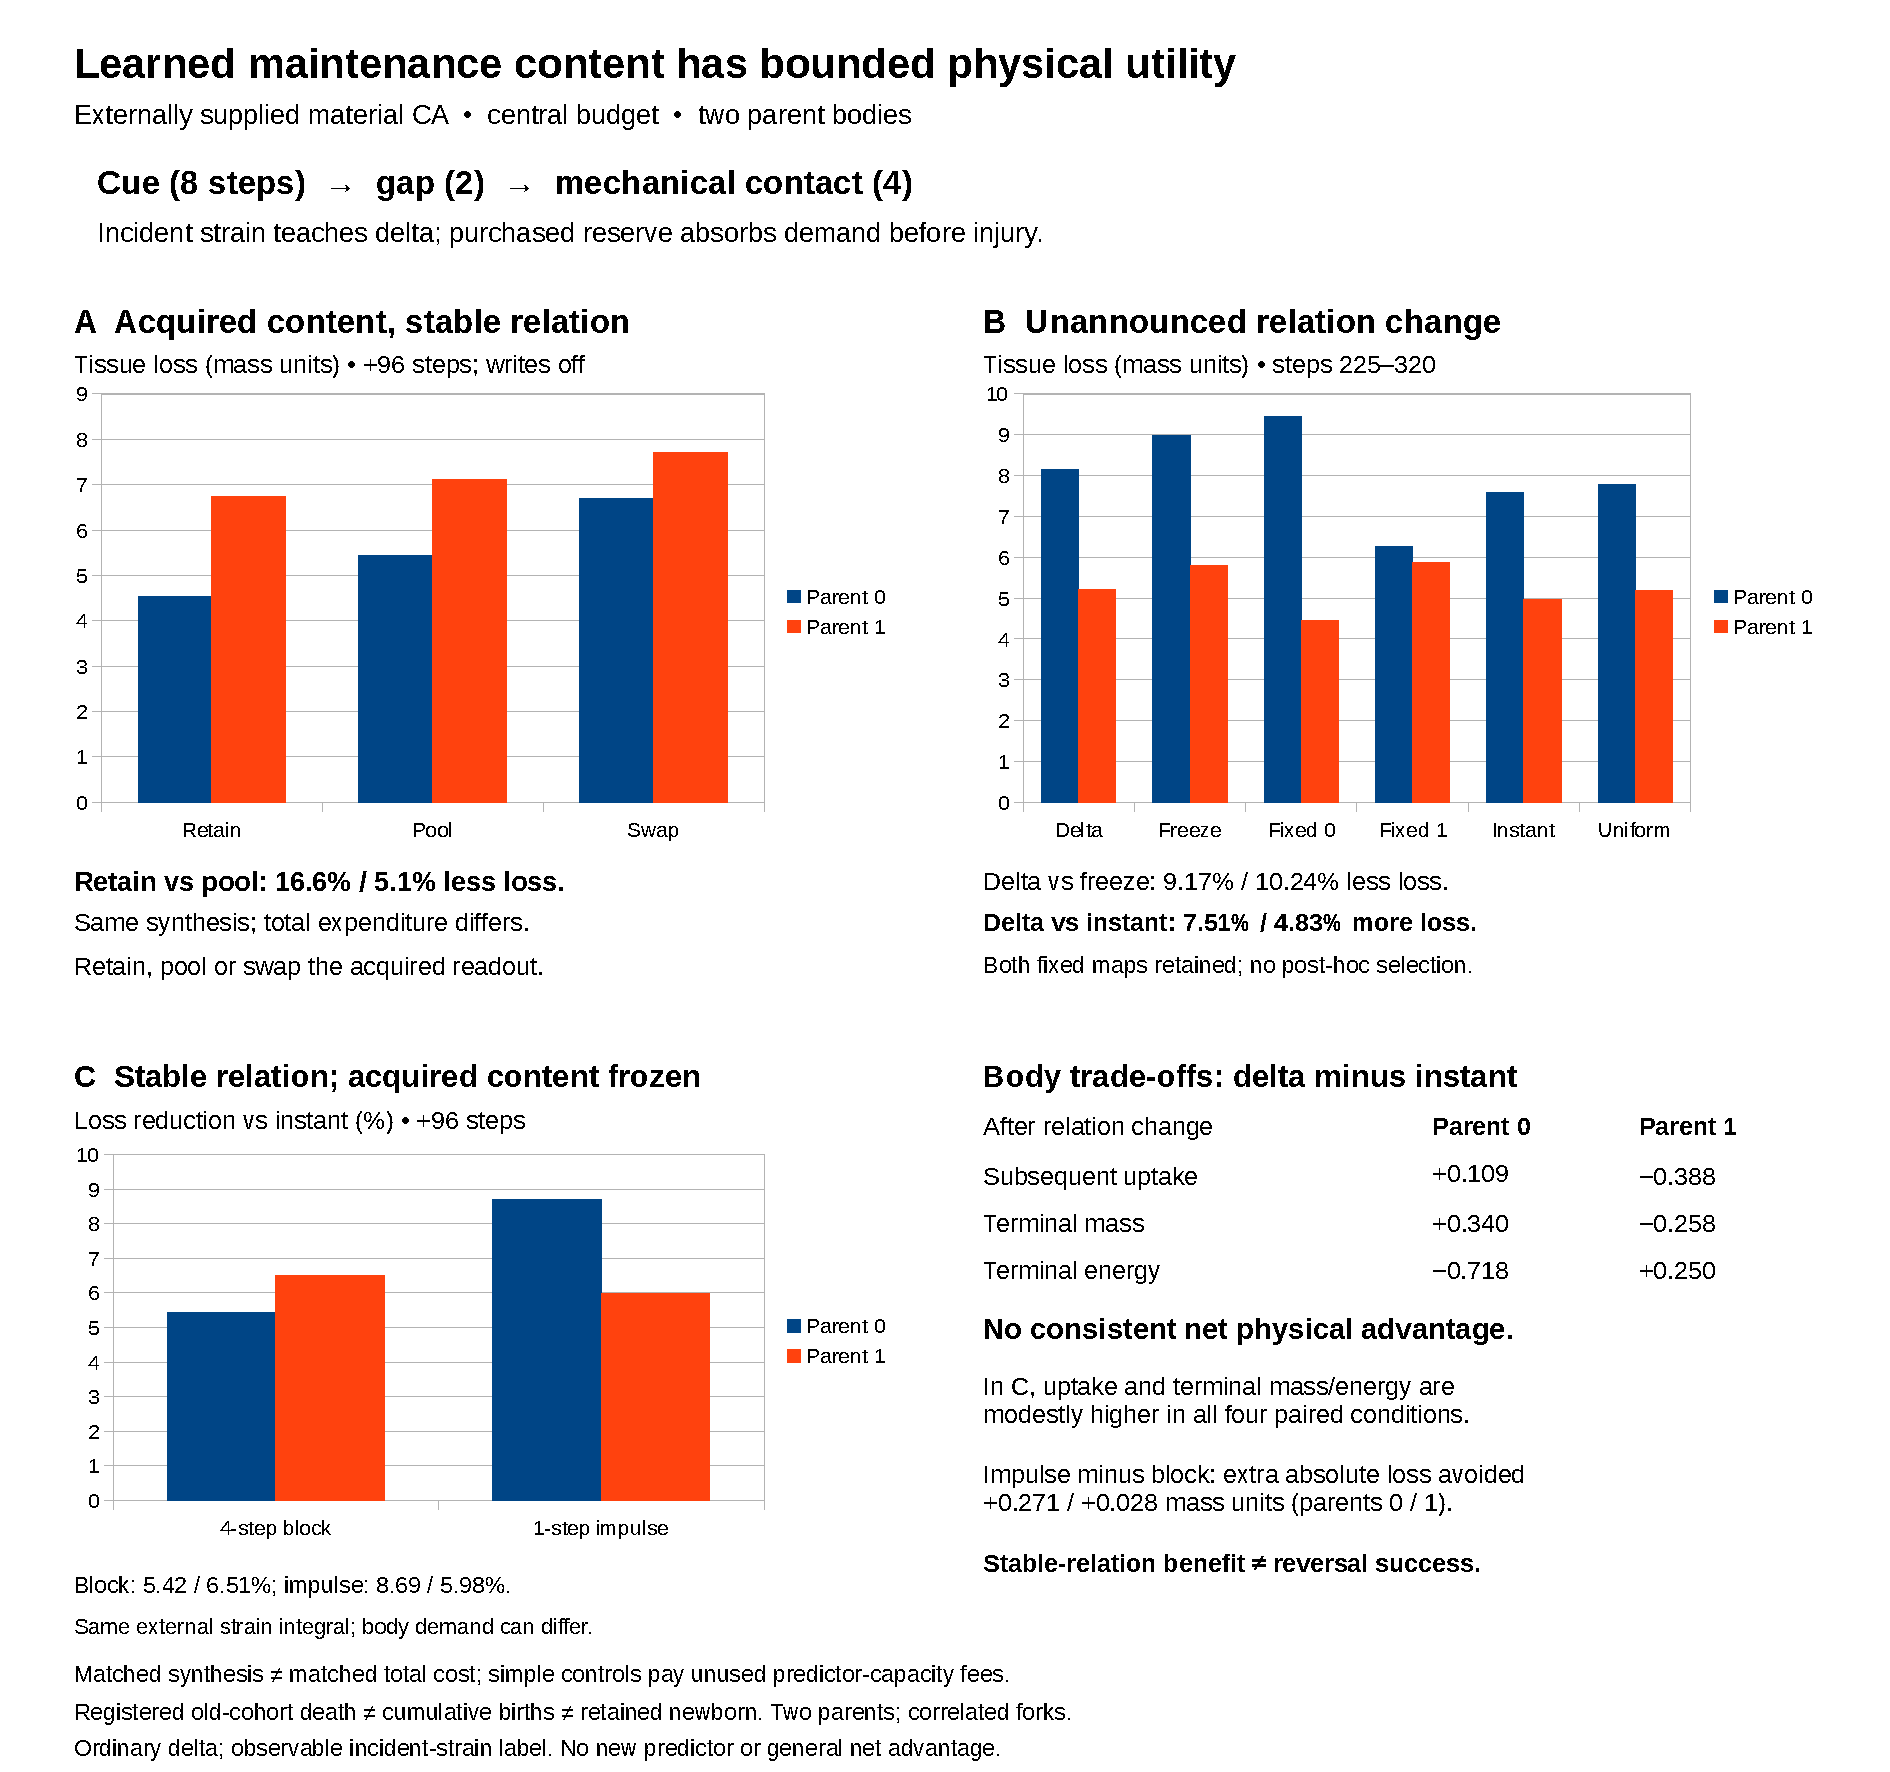
\includegraphics[width=\linewidth,height=0.63\textheight,keepaspectratio]{work/longform_v047/figures/predictive_maintenance_v048/predictive_maintenance.pdf}
\captionsetup{font=footnotesize}
\caption{\textbf{Acquired conditional maintenance has limited physical utility against strong instantaneous controls.}
The externally supplied, density-regulated material CA has centrally coordinated purchasing and a local incident-strain sensor. The ordinary conditional delta rule learns from completed contact, including strain absorbed by reserve; it is not a new predictor.
\textbf{a}, All three content readouts of two acquired parents over 96 new steps with writes stopped and the learned relation retained. Retaining rather than pooling content reduces injury by 16.6\%/5.1\% at equal realized reserve synthesis; swapping also raises injury.
\textbf{b}, All six policies from both actual parents. Bars show injury in steps 225--320 after the relation changes at boundary 224. Continued delta reduces injury relative to frozen content by 9.17\%/10.24\%, but loses 7.51\%/4.83\% more tissue than the instantaneous rule. Neither fixed map is selected retrospectively. The accompanying delta-minus-instantaneous contrasts show opposed uptake and terminal mass/energy effects, without consistent net benefit.
\textbf{c}, Two actual 192-step parents each supply four 96-step futures under the retained relation, crossing block/impulse contact with acquired/instantaneous readout; writes are frozen. External strain integrals match, while realized bodily demand can differ. Bars show paired injury reductions relative to instantaneous allocation. The impulse increases the absolute avoided-loss contrast by 0.271/0.028 mass units, but proportional benefit does not rise in both parents. This is a stable-relation expression test, not reversal success or isolation of one timing mediator.
Colours identify source parents within each assay; their branches are correlated conditions. Equal synthesis does not equalize total expenditure. Simple controls carry unused predictor capacity and its fees. Old-cohort death, cumulative birth and retained newborn tissue are distinct; none establishes newborn-content necessity. The original missing risk tail is not imputed. Full phase outcomes and physical accounts are in the accompanying maintenance source tables.}
\label{fig:predictive-maintenance}
\end{figure}


